\documentclass{article}
\usepackage{tikz,lipsum,lmodern}
\usepackage[english]{babel}
\usepackage[most]{tcolorbox}
\usepackage[paperheight=10.75in,paperwidth=7.25in,margin=1in,heightrounded]{geometry}
\usepackage{graphicx}
\usepackage{blindtext}
\usepackage{ragged2e}
\usepackage{needspace}
\usepackage[space]{grffile}
\usepackage[utf8]{inputenc}
\usepackage[export]{adjustbox}
\usepackage{hyperref}
\usepackage{placeins}
\usepackage{fancyref}

\hypersetup{
    colorlinks,
    citecolor=black,
    filecolor=black,
    linkcolor=black,
    urlcolor=black
}
\usepackage{chngcntr}
\counterwithin{figure}{section}

\usepackage{fancyhdr}
\pagestyle{fancy}
\fancyhf{}
\rhead{\rightmark}
\chead{\thepart}
\lhead{\nouppercase{\leftmark}}
\cfoot{\thepage}
\graphicspath{{"./img/"}}

%\setcounter{secnumdepth}{3} % default value for 'report' class is "2"
%\setcounter{tocdepth}{3}

\newcommand{\lbl}[1]{(see image \ref{#1})}
\newcommand{\img}[1]{
	\centering
	\includegraphics[max width=.9\textwidth]{#1.png}
	\label{#1}
}

\title{%
Neural Networks \\
\large Deep Learning}

\author{Silas Hoffmann, inf103088}
\date{\today}


\begin{document}
\maketitle

\vspace{0.5cm}
\tableofcontents
\vspace{0.5cm}
\listoffigures
\vspace{0.5cm}

\section{Introduction}
Notes for the introduction to neural networks presented by \textbf{3blue1brown}. Watch the whole series here: \href{https://www.youtube.com/watch?v=aircAruvnKk}. This series describes the strategy to recognize handwritten numbers.

\clearpage

\section{Chapter 1 - But what is a neural network?}

% -------------------------------------------------- 

\subsection{Structural overview}

\FloatBarrier

\begin{figure}[h]
\img{ai_1}
\caption{Image interpreted as first layer of neural network}
\end{figure}

Each pixel from the image is represented by a so called \textit{neuron} \lbl{ai_1}. These neurons possess a value called \textbf{Activiation} which contains a float between 0 and 1. This value specifies the brightness of this the particular pixel. This activation value also can be interpreted as how \textit{lit up} this particular neuron actually is, 1 meaning 100 \% in this context.


\begin{figure}[b!]
\img{ai_2}
\caption{Resulting top layer}
\end{figure}

As each number is analyzed the top layer gives its prediction to a given input via Activation of the ten most right nodes \lbl{ai_2}. The one with the highest activation states what the system thinks the correct number might be. The layers between the top and the bottom layer are called \textbf{hidden layers}. 

\begin{figure}[h]
\img{ai_3}
\caption{Image interpreted as first layer of neural network}
\end{figure}

The number of layers is not fixed and can be set to any number appropriate to the problem the system should solve. In this example it is useful to two hidden layers because of how the system works. A handwritten digit can be subdivided into different components \lbl{ai_3}. E.g. the number 9 can be divided into a top loop and a bottom line. These different steps will be analyzed by the various layers from the network. Maybe some digits share specific components and those nodes can be \textit{reused} \lbl{ai_4}. The idea is that any digit with a \textit{loopy} pattern towards the top sends of the specified neuron. This information is then used to fire up neurons in the next layer based on the idea that at least some kind of pattern already fits the input data.

\begin{figure}[h]
\img{ai_4}
\caption{Recognizing more complex patterns via abstraction}
\end{figure}

But to be capable of recognizing such a complex patterns as a loop, the system has to recognize all the various subcomponents of a loop. Those mainly consist out of small edges which in total form a loop from a wider perspective. This may be the task of the second layer while the third layer is responsible for recognizing those more complex parts \lbl{ai_6}. 

Again, the number of layers is totally arbitrary. It might even be usefull to divide those smaller lines from layer 2 into smaller components, then there might be another layer. Or maybe the second layer is redundant altogether because the system can recognize those complex pattern directly. It always depends on the problem that the network should solve to decide how many layers are actually usefull.

\begin{figure}[h]
\img{ai_5}
\caption{Examples of simple shapes forming complex digits}
\end{figure}

In a nutshell the different layers in a neural network each describe a certain level of complexity. Those lower levels represent simpler coherence than the ones on top of those. In the next picture you can see the which neurons on each layer may fire when confronted with a sample of a handwritten nine.

\begin{figure}[h]
\img{ai_6}
\caption{Top to bottom overview}
\end{figure}

% -------------------------------------------------- 

\subsection{Regognizing patterns}
The main purpose of the given example network is to detect edges of the given digits and from these edges determine patterns which in turn result in a identified digit. But this principle of detecting details and forming a bigger picture is also relevant in other fields e.g. autonomous cars or speeach regognition where a given audio samples consists out of waves which form voices which form words etc. 

To show how it actually works to detect one of those minor details to from the simples \textit{hidden layer} the tutor shows how to recognize a single line in a specific part of the picture \lbl{ai_7}.

\begin{figure}[h]
\img{ai_7}
\caption{Bounding box for detecting specific line}
\end{figure}

\begin{figure}[h!]
\img{ai_8}
\caption{Colored weights for specifying outlines}
\end{figure}

In the example we try to detect the middle part of the digit seven \lbl{ai_8}. To check whether or not the given pixels have a line in the specified part of the image we assign a so called \textbf{weight} to each of the connections of nodes on the first layer (direct image input) to the node responsible for recognizing the depicted part of the image as a line. To do so each connection outside of the bounding box gets assigned a value of zero and the relevant nodes get a value greater zero. Now each weight will be multiplied with the corresponding node value \textit{(brightness of the node)} and all those values will be added. Whenever there is actually a line in the specified box the sum of the values will be higher than if there wasn't a line. To make it state that we actually expect a line which does not touch the upper and lower bound of the box we can also create negative bounds for the outer pixels which in turn extravagates the result even more. 

E.g. a black line crosses the otherwise completely blank / white canvas. Then the nodes which are expected to be white multiply by a quite big factor with the small values and the outer pixels touch the bound of the box. This will result in some pretty huge negative numbers because the weight are negative in those places. On the other hand, if you put a perfect line that is not touching the bounds in the box then the sum of all products with the weights will be much larger and the neuron will fire a value much \textit{\textbf{brighter}}.

\begin{figure}[h]
\img{ai_9}
\caption{Sigmoid function}
\end{figure}

Since the calculated sum of the product with the weights may very well be much larger than 1 or smaller than 0, the sum will be squished into the the interval 0 to 1 via some kind of function. Often a function called the \textbf{sigmoid function} is used which creates a value near zero for negative values and a value near 1 for high values \lbl{ai_9}. It is important to limit the output to this interval because it will serve as the \textbf{activision} of the node when the node is used in the next step / layer of the network. 

A very important summary: \textit{The activation of a neuron is basically a measure of how positive the relevant weighted sum is.}


\begin{figure}[h]
\img{ai_10}
\caption{Activation displayed with bias and sigmoid function}
\end{figure}

Another important tool is the so called \textbf{bias} which acts a sort of lower bound for the activation of the neuron. Say you want the neuron to only detect very thick and bright lines. Then you need this bias to to say something like \textit{only light up when weighted sum is greater than 10} \lbl{ai_10}. This can be achived by subtracting the bias inside the sigmoid function.


\begin{figure}[h]
	\centering
	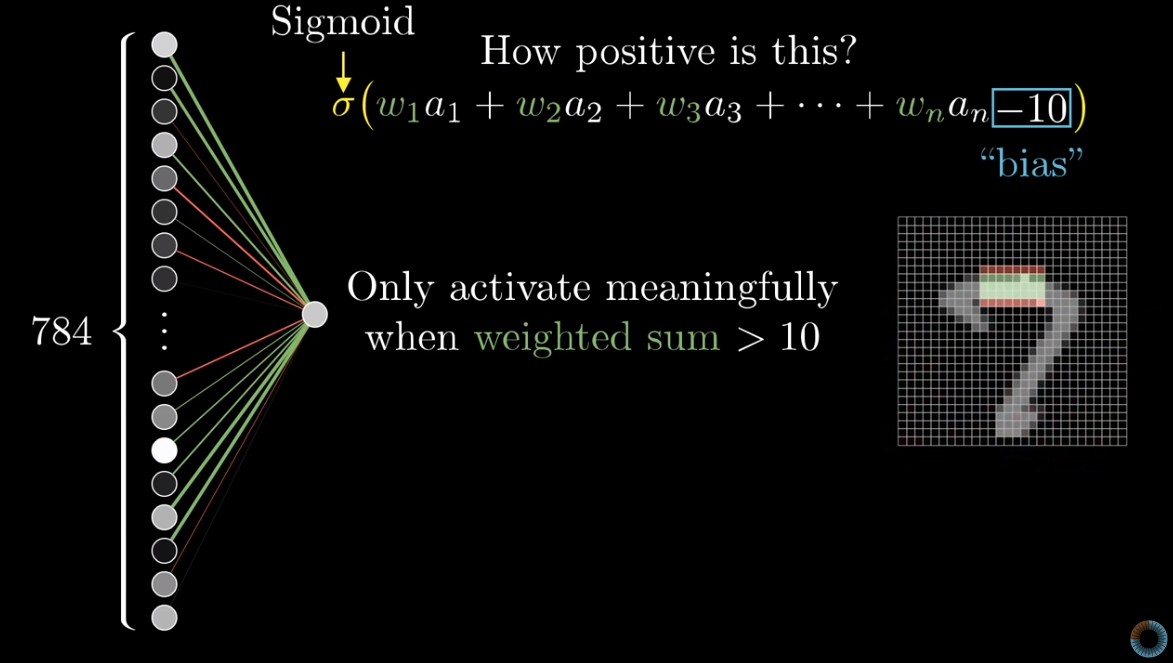
\includegraphics[max width=.9\textwidth]{ai_10.png}
	\label{fig:ai_10}
\end{figure}

\ref{fig:ai_10}
%\ref{fig:ai_10} \autoref{fig:ai_10}

\end{document}

